\documentclass[twocolumn]{article}

\usepackage{bm}
\usepackage{graphicx}
\usepackage{amsmath}
\usepackage{amssymb}
\usepackage[hyphens]{url}
\usepackage{multirow}

\begin{document}	
	\twocolumn[
	\begin{@twocolumnfalse}
		\author{Mohamed Moanis Ali, Michael Sedrak \\  mohamed.moanis.ali@gmail.com, m.sedrak@live.com}
		\title{Comparative Analysis of Approximation Algorithms for Solving TSP}
		\maketitle
		\begin{abstract}
			The traveling salesman problem is considered one of hardest problems in computer science with no polynomial runtime algorithm to solve it so far. Nevertheless, TSP is an active research point with more algorithms being developed to either approximately solve the original problem, or to speed it up so larger datasets can be solved. In this work we present a comparative study using four algorithms to solve TSP -genetic algorithm, simulated annealing, nearest neighbor and ant colony optimization to analyze the runtime performance and the correctness of their solution.  The results of the experiments on the Uruguay dataset -using both {Matlab\texttrademark}  and Octave- showed that the nearest neighbor algorithm provided the fastest runtime and a relatively correct solution with $18\%$ from the known optimal solution, while the ant colony optimization proved to be the least correct among the studied algorithms. The study also found a huge performance difference between {Matlab\texttrademark}  and Octave software.
		\end{abstract}
		
	\end{@twocolumnfalse}
	]
	
	%% Document body starts from here
	
	\section{Introduction}
	The traveling salesman problem (TSP) is a classical combinatorial optimization problem with a long history -dating back to 1832, and countless number of real life applications\cite{applegate07}\cite{punnen07}. It was first mentioned in a handbook for traveling salesmen in Germany and Switzerland to be mathematically formulated later in 1930. Though easy to describe, TSP is a NP-hard problem; that's it, there is no polynomial time algorithm to solve it. This limits the use of exact methods which have a time complexity of $O(n!)$ to a small number of cities.
	
	The problem is to find the shortest route between a given set of cities' locations where each city must be visited only once and the trip must end by returning back to the starting city. TSP can be modeled as an undirected weighted graph, such that cities are the graph's vertices and paths between cities are the graph's edges. The distance between two given cities in both direction can be the same which is called symmetric TSP and can differ in case of asymmetric variant. In this work, we will only consider the symmetric TSP.

	The optimization problem to solve TSP can be formulated as a linear programming problem as follows\cite{papadimitriou98}:
	\begin{equation} \label{eq:TSPLinearProgramming}
	min \sum_{i=1}^{n} \sum_{j=1, j\neq i}^{n} {c_i}_j {x_i}_j
	\end{equation}
	where ${c_i}_j$ is the cost between cities $i$ and $j$ and ${x_i}_j$ is given by Eq.(\ref{eq:TSPX})
	\begin{equation} \label{eq:TSPX}
	{x_i}_j = 
	\begin{cases}
	1,& \text{path goes from i to j}\\
	0,& \text{otherwise}
	\end{cases}
	\end{equation}
	The complexity of TSP, makes room for approximate algorithms to arise\cite{Brucal17}. Such algorithms can reach near optimal solution in a reasonable time as seen in this work. Algorithms such as variable neighborhood search\cite{Thanh15}, genetic algorithm\cite{Wang17}, monte-carlo trees search\cite{Perez14}, adaptive bee colony\cite{Rekaby13}, meta-learning\cite{Kanda11}, machine learning\cite{Pihera14}, simulated annealing\cite{Kerrache14}, ant colony optimization\cite{Swiatnicki15}, harmony search\cite{Tongchan17}, biography based approximation\cite{Wu17} and variations of neural networks\cite{Gao10}\cite{Mueller15} have addressed the TSP. In this work we will focus on four of such algorithms, namely: genetic algorithm\cite{Kirk14}\cite{mathwork}, simulated annealing\cite{Jang02}, nearest neighbor search\cite{Jevtic14} and ant colony optimization\cite{Ibrahim15}. This survey will compare {Matlab\texttrademark}  implementation of the four algorithms in terms of runtime performance and how close they are to the optimal solution.
	
	\section{Dataset}
	Datasets for TSP problem contain a wide variety of formats. Cities across a country, VLSI nodes or traveling across the Mona Lisa drawing. But they are all similar in the aspect of the data structure. The structure is a 2-D coordinate point system with euclidean distances as the distance between nodes.
	For our work we selected the Uruguay dataset from the national dataset collection\cite{UY734} to be used to assess the four algorithms in this survey in terms of runtime performance and how close is their solutions compared to the dataset know optimal solution. Uruguay dataset is characterized by 
	\begin{itemize}
		\item 734 unique points (no duplicates)
		\item Optimal tour of length 79114
	\end{itemize}
	\begin{figure}[h!]
		\centering
		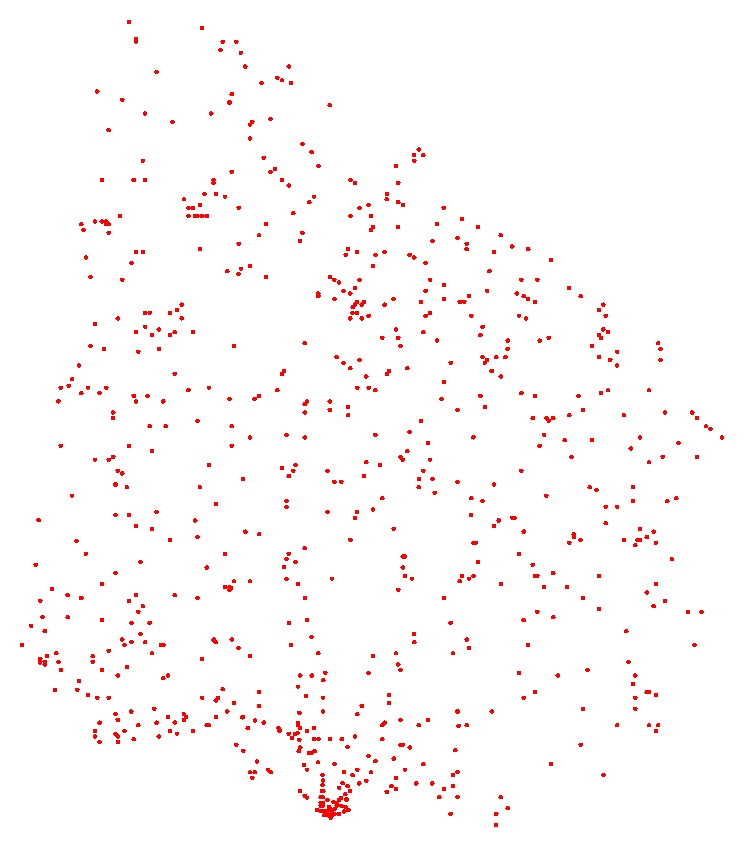
\includegraphics[scale=0.3]{./uypoints.jpg}
		\caption{XY coordinate representation of Uruguay dataset}
		\label{fig:uruguay}
	\end{figure}
	A graphical representation of the coordinates of the dataset is shown in figure \ref{fig:uruguay}
	
	\section{Algorithms}
	In this section, the four algorithms are considered with a brief description of how they solve the TSP problem.
	\subsection{Genetic Algorithm}
	
	Genetic algorithm (GA) is a randomized metaheuristic search technique that simulates the process of evolution and natural selection in order to solve combinatorial optimization problems. Operations like mutation, crossover and selection are used to search for the optimal solution for a given problem.
	
	Genetic algorithm formulates a problem using the same terminology that is used in the biological process of evolution. A population of candidate solutions -each individual solution is called individual- is evolved toward an optimal solution. In the evolutionary iterative process, each individual is assessed to measure its fitness score using an objective function. The individuals with higher score are selected to have their genes or DNA mutated and changed which will result in a new population of possible solutions. The process goes on until an individual with a satisfactory fitness score is reached or the maximum number of generations has been produced.
	
	TSP can be easily formulated in GA context. The search space is the set of routes that spans all the cities of Uruguay, and the goal is to find a route with the minimum cost. Each route is considered as an individual with a DNA that resembles the ordered set of towns and cities in the route -genes. The mutation and crossover of individuals is the process of reordering genes in an individual's DNA to produce new individuals. The solution for TSP will be an individual with DNA representing the optimal route between towns and cities that have the minimal distance cost.
	
	The iterative process for solving TSP using GA is given by the following steps:
	\begin{enumerate}
		\item Create an initial population of size (N=100).
		\item Evaluate the fitness of each individual in the population.
		\item Select (M=4) individuals from the current population using their fitness score as a criterion.
		\item Mutate selected individuals and create 3 new routes.
		\item Repeat steps 3 and 4 until all the individuals are mutated.
		\item Replace the old population with the new mutated one.
		\item Go back to step 2 if more generations can be mutated or the number of iterations did not reach an upper bound of iterations. Otherwise, the final result is the best population created and the most fit individual is considered TSP solution.  
	\end{enumerate}
	It is important to note that the resultant solution is not necessarily the optimal one. Specially, when a limited number of GA iterations is used to reduce the relatively large calculation time to be able to converge to the optimal solution.
	
	\subsection{Simulated Annealing}
	Simulated annealing (SA) is another algorithm that mimic a natural phenomena; this time it is the heat treatment process used on metals. During the annealing process, a metal is heated enough to allow its molecular structure to be altered. The temperature {\bfseries T} is steadily lowered by a cooling constant {$\boldsymbol \beta$}, which subsequently lowers the energy of the atoms and restricts their arrangement until the metal's structure finally becomes set. That in turn, minimizes the number of defects in the structure of the metal.
	 
	SA can be considered as a modification for greedy search as an attempt to reach an optimal solution rather than getting stuck at a local optimum. For example, consider a problem of searching a function with the goal of reaching the global optimum. A greedy approach would move in the direction that result in a higher gain and stops once no more moves would lead to a higher gain, thus, a greedy approach can miss the global optimal solution.
	 
	In contrast to greedy approach, SA occasionally allows moves in directions with lower gain that would not have been accessible otherwise. SA starts at random solution -a state {\bfseries S}- and then at each iteration step, the solution is slightly modified in order to choose another search point and move to a new state $\boldsymbol{S\prime}$. This modification is made with a random reorder of a constant number of elements in the solution space {\bfseries M}. The selection process of the new state -solution- considers the change in cost {\bfseries C} - know as {$\boldsymbol \gamma$}- that will be incurred if the new state is chosen. When the cost is going to be lower, the new state is chosen. Else, however, the incurred cost might increase there is still a chance to accept this state with a probability \\{\bfseries P({$\boldsymbol \gamma$}, T)} that is relative to the current temperature of the simulation; that's it, when the current temperature is high, the probability to take worse solutions will be higher as there still more simulation time available to try different search point in order to reach the global optimum.
	 
	In the context of TSP, each state in SA algorithm is a route between the towns and cities. The cost measured for each route is the distance  between its points and accordingly the optimal solution is that with the minimum distance. SA algorithm would then work in the following steps:
	\begin{enumerate}
		\item Choose random state {\bfseries S} and the starting temperature {\bfseries T} and cooling constant {$\boldsymbol \beta$}.
		\item Create new state $\boldsymbol{S\prime}$ by randomly swapping {\bfseries M} cities in the current state.
		\item Compute the change in cost using Eq.(\ref{eq:GADelta})
		\begin{equation} \label{eq:GADelta}
		\gamma = \dfrac{C(S')-C(S)}{C(S)}
		\end{equation}
		\item If {$\boldsymbol{\gamma \leqslant 0}$, then {\bfseries S =} $\boldsymbol{S\prime}$.}
		\item Else, compute the probability using Eq.(\ref{eq:GAProb})
		\begin{equation} \label{eq:GAProb}
		P(\gamma, T)=
		\begin{cases}
		1,& \text{if } \gamma\leqslant 0\\
		e^{\frac{-\gamma}{T}},& \text{otherwise}
		\end{cases} 
		\end{equation}
		\item Randomly assign {\bfseries S =} $\boldsymbol{S\prime}$ using {$\boldsymbol \gamma$}.
		\item Repeat steps 2 to 6 until stopping conditions are met; ie, temperature reaches a certain threshold or a required number of iterations is met.
	\end{enumerate}
	Finally, the performance of SA can be controlled by the choice of the initial temperature, cooling constant and the number of cities modified in each step. Additionally, the stopping conditions are of quite importance for SA to reach a near optimal solution. If the algorithm is stopped too soon, the approximation will not be as close to the global optimum. And if the algorithm is not stopped soon enough, more time will be wasted on calculations and search steps with little to no gain.

	\subsection{Nearest Neighbor (NN)}
	Nearest neighbor approach is one of the simplest algorithms in combinatorial optimization problems and also one of the fastest running algorithms\cite{GreedyNN}.
	
	The algorithm implementation for solving the TSP problem is as follows:
	\begin{enumerate}
		\item Select a random city as the current city
		\item For all cities
		\item Select the closest unvisited city to the current one
		\item Mark current city as visited
		\item Visit the new selected city
		\item If all cities are visited then terminate
		\item O.W. go back to step 3
	\end{enumerate}
	
	The NN approach is greedy in nature, usually resulting in a non optimal solution. It can miss shorter routes that might be noticed with human sight. Based on the distribution of cities, the NN approach may provide the optimal solution.
	
	\subsection{Ant Colony Optimization (ACO)}
	The Ant Colony Optimization (ACO) algorithms tries to mimic the natural phenomenon of ants finding a path from a food source to the colony. Ants start first going at random paths in the paths, leaving trails of a chemical substance called pheromone behind. Pheromone evaporates with time, therefore shorter paths tend have heavier trails of pheromone as they are marched more frequently thus attracting more ants to this path. Since pheromone evaporates this provides an advantage of avoiding the convergence to a local minimum path. In other words, if pheromone did evaporate at all, the paths chosen by the first ants would still attract the following ants.
	
	\begin{figure}[h!]
		\centering
		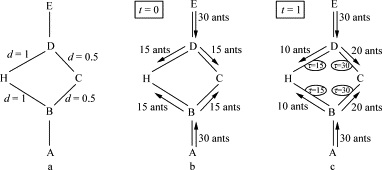
\includegraphics[scale=0.8]{./ACOexample.jpg}
		\caption{ACO example\cite{ACOExample} (a)The initial description of the problem showing distances. (b)At time t=0 no trail is found on the graph therefore ants choose the paths with equal probability. (c)Trails from previous step are found and therefore the choice of paths is biased towards the shorter edges.}
		\label{fig:ACOexample}
	\end{figure}
	
	For better understanding of the ACO algorithms, an example from\cite{ACOExample} is illustrated. As shown in Fig.\ref{fig:ACOexample} a, the system is shown with the initial start points A as the food source ,and E as the colony nest, and the distances of the paths. At t=0, 30 ants start moving from both E and A simultaneously. The ants currently can see no preference between the different paths because there are no traces of pheromone left behind, therefore, the ants divide randomly with equal probability going in to both points H and C, i.e. 15 ants are going from D to C and 15 ants from D to H, and similarly from point B to both C and H. At t=1, the 30 new ants coming from B, find 2 unequal paths, the path going to H has a trail of 15 from the ants that went to H from B, while the path going to C has a trail of 30 that can be divided into:
	\begin{enumerate}
		\item The trail from ants going from point B.
		\item The trail from ants coming from point D.
	\end{enumerate}
	 Resulting in a bias in the probability of choosing the path unlike the previous step. The number of ants going to C is expected to be double the number of ants going to H. The same is true for the 30 new ants coming from D.
	
	In combinatorial problems\cite{ACO}, we deal with simulated virtual ants. These virtual ants differ than the real world ants in two aspects.
	\begin{enumerate}
		\item Artificial ants have a prior knowledge of the distances between cities and therefore tend to select the shorter distance.
		\item Artificial ants have memory, they know which cities they have visited along a path and will not select those cities again.
	\end{enumerate}
	We can express the probability of ant \textit{k} selecting city \textit{j} after city \textit{i} as follows:
	
	\begin{equation} \label{eq:ACOprobability}
		\textit{p}^\textit{k}_\textit{ij} = 
	\begin{cases}
	{\dfrac{[\tau_{ij}]^\alpha \textbf{.} [\eta_{ij}]^\beta}
		{\sum_{s \in allowed_k} [\tau_{is}]^\alpha \textbf{.} [\eta_{is}]^\beta}  } ,& \text{if } \textit{j} \in \textit{allowed}_k
	\\
	0,& \text{otherwise}
	\end{cases}
	\end{equation}
	where:
	\begin{itemize}
		\renewcommand{\labelitemi}{-}
		\item $\textit{p}^\textit{k}_\textit{ij}$ is the probability that city \textit{j} will be selected after city \textit{i} by ant \textit{k}.
		\item $\tau_{is}$ is the intensity of pheromone between cities \textit{i} and \textit{j}.
		\item $\alpha$ is the parameter to regulate the influence of trails of pheromone.
		\item $\eta$ is the visibility of city \textit{j} from city \textit{i} which is always measured as $\dfrac{1}{\text{distance between cities \textit{i} and \textit{j}}}$.
		\item $\beta$ is the parameter to regulate the influence of $\eta_{ij}$
		\item allowed$_k$ is the set of unvisited cities.
	\end{itemize}

	At the beginning of the algorithm, \textit{N} ants are assigned initial starting points (cities) at random. As the iterations proceed, ants decide which cities to visit according to $\textit{p}_\textit{ij}$ described in Eq. (\ref{eq:ACOprobability}). After \textit{n} iterations, each ant completes a tour. Tours with shorter distances, have stronger pheromone trails. Therefore updating the trails follow \textit{Q}/\textit{L}$_\textit{k}$ where \textit{Q} is a constant value and \textit{L}$_\textit{k}$ is the path length. Also as we mentioned before the pheromone trails evaporate with time. Therefore we can update $\tau_{is}$ according to the following equations:
	
	\begin{equation} \label{eq:ACOTrailUpdate1}
		\tau_{ij}(t+1) = \rho \textbf{.} \tau_{ij}(t) + \Delta\tau_{ij}
	\end{equation}
	
	\begin{equation} \label{eq:ACOTrailUpdate2}
		\Delta\tau_{ij} = \sum_{k=1}^l \Delta\tau_{ij}^k
	\end{equation}
	
	\begin{equation} \label{eq:ACOTrailUpdate3}
	\Delta\tau_{ij}^k = 
	\begin{cases}
	\textit{Q}/\textit{L}_\textit{k},& \text{if ant k travels the path (\textit{i}, \textit{j})}
	\\
	0,& \text{otherwise}
	\end{cases}
	\end{equation}
	
	where:
	\begin{itemize}
		\renewcommand{\labelitemi}{-}
		\item \textit{t} is the iteration counter.
		\item $\rho$ $\in$ [0,1] the parameter to regulate the reduction of $\tau_{ij}$.
		\item $\Delta\tau_{ij}$ is the total increase of pheromone trail on the edge (\textit{i},\textit{j})
		\item $\Delta\tau_{ij}^k$ is the increase of pheromone trail caused by ant \textit{k}.
	\end{itemize}	
	The algorithm to solve TSP with ACO is as follows:
	
	\begin{itemize}
		\item For i=1 to iteration number
		\begin{itemize}
		\item For k=1 to number of ants
			\begin{itemize}
			\item While no complete tour is found by ant k
				\begin{itemize}
				\item Select city j to be visited according to Eq.(\ref{eq:ACOprobability})
				\end{itemize}
			\item Calculate L$_k$
			\end{itemize}
		\item Update pheromone trail levels according to Eqs.(\ref{eq:ACOTrailUpdate1},\ref{eq:ACOTrailUpdate2},\ref{eq:ACOTrailUpdate3}).
		\end{itemize}
	\end{itemize}
	
	\section{Results}
	The codes to solve the TSP problem [links!!!] were executed on both Matlab and Octave, taking into consideration the resulting output path length and the execution time. All the test conducted were repeated ten times each in order to see how well the algorithms can improve in both criteria. In the program using GA, the running time on Octave was 45,362 seconds (approximately 12.5 hours). Due to the long duration of the test runtime this experiment was not repeated except two times. While the running time on Matlab provided a minimum time of 76 seconds on the first trial and a maximum time of 118.9 seconds on the 8$^th$ trial, the shortest path found was on the 6$^th$ iteration, of length 226,854.7 which is 65\% within the optimal solution. While the optimized GA algorithms produced much better running times for the same number of iterations with a minimum of 23.8 seconds on th first run and a maximum of 32.1 seconds on the 7$^th$ run, the final path length didn't differ much from the previous implementation, a path of length 200068 was found which is 60\% within the optimal solution. At a much faster running time and a slight improvement of 5\%, the seconds GA algorithm can be run for longer iterations and thus providing much better results. Results of GA run is shown in fig.\ref{fig:GAalgorithm}
	
	\begin{figure}[h!]
		\centering
		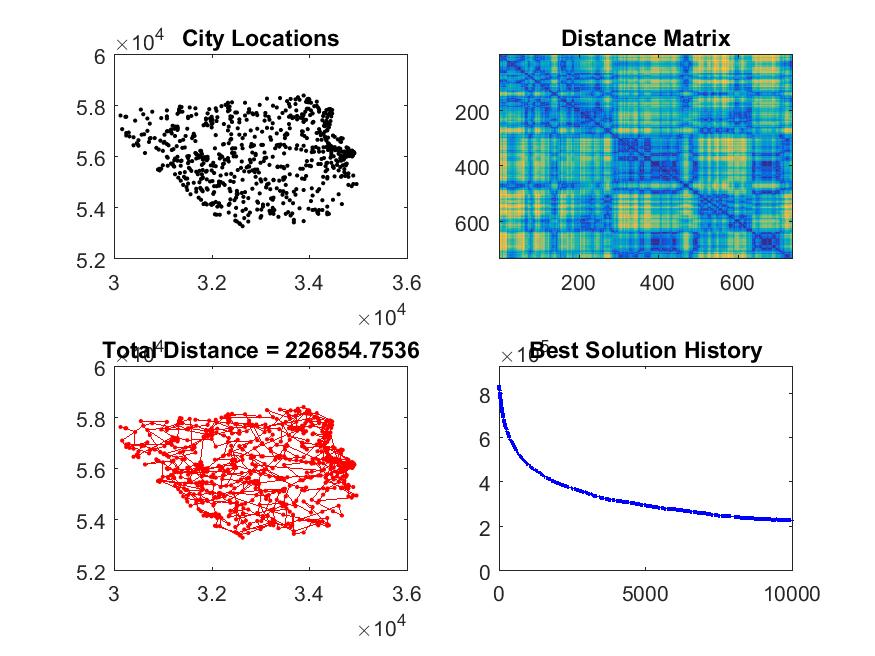
\includegraphics[scale=0.25]{./GA1.jpg}
		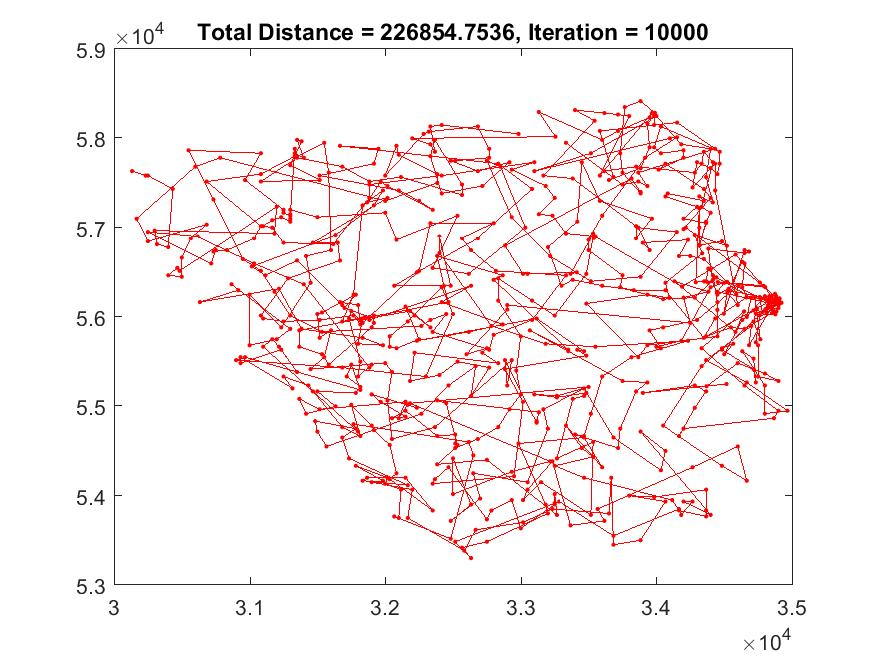
\includegraphics[scale=0.25]{./GA2.jpg}
		\caption{TSP using GA algorithm}
		\label{fig:GAalgorithm}
	\end{figure}
	
	Simulated annealing approach tested on Octave produced a minimum running time of 1217 seconds at the 4$^th$ test and a maximum of 1526.3 seconds at the 10$^th$ test, while on Matlab a minimum of 62.8 seconds and a maximum of 107.5 seconds running times were produced on the first and last tests respectively. The shortest path solution produced to our dataset was of length 89237 which is within 11.34\% of the optimal solution.
	
	The nearest neighbor tests conducted on Octave provided running times ranging between 132 seconds and 136 seconds, which are approximately 7 to 10 times less than all other conducted tests of different algorithms. On Matlab, the tests took 10.8 seconds for the quickest run and 15.4 seconds for the longest run on the 1$^st$ and 5$^th$ runs respectively. The nearest neighbor implementation conducted did not take a random starting point and therefore all runs provided the same path length of 96,514.8 which is approximately 18\%  within the optimal solution. Results of NN run is shown in fig.\ref{fig:NNalgorithm}
	
	\begin{figure}[h!]
		\centering
		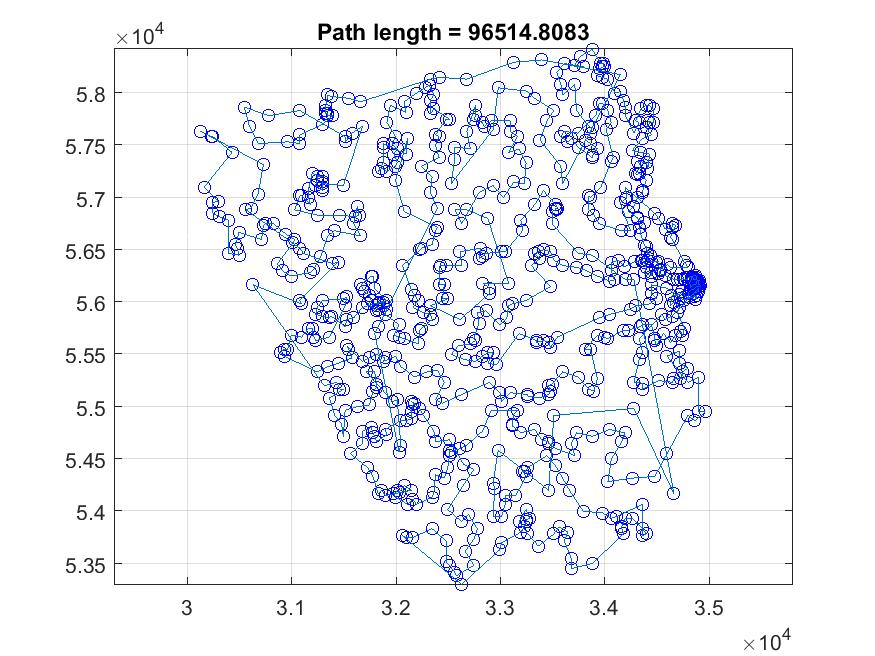
\includegraphics[scale=0.25]{./NN.jpg}
		\caption{TSP using NN algorithm}
		\label{fig:NNalgorithm}
	\end{figure}
	
	The ant colony tests resulted in running times between 777.8 seconds and 790 seconds on Octave and between 11.7 seconds and 16.8 seconds on Matlab. The algorithm default parameters used runs the algorithm for 10 iterations and the shortest path length found was of length 951387 and that is 91.5\% within the optimal solution. A run for 100 iterations was conducted. This took 130 seconds to complete and provided a path of length 880279, 91\% within the optimal solution and 0.5\% better than the previous run.
	
	The previous results are tabulated in Table \ref{tab:results}
	

	\begin{table}[h!]
		\caption{Results of TSP algorithms}
		\scalebox{0.8}{
		\begin{tabular}{cccccc} 
			\hline
			{Algorithm} &{GA} &{SA} & {NN} & {ACO} &{OGA}\\
			
			\hline
			{\multirow{2}{*}{Octave}} & {45362} &{1217}& {132} &{777} &{N/A} \\
			 running time & & & & & \\
			 
			\hline
			{\multirow{2}{*}{Matlab}} & {76} &{63}& {11} &{12} &{24} \\
			running time & & & & & \\
			
			\hline
			{\multirow{2}{*}{Generated}} & {226854} &{89237}& {96514} &{951387} &{200068} \\
			path length & & & & & \\
			
			\hline
			{\multirow{2}{*}{Efficiency}} & {65\%} &{11.3\%}& {18\%} &{91.5\%} &{60\%} \\
			of path & & & & & \\
			
			\hline
		\end{tabular}}
	\label{tab:results}
	\end{table}

	
	\section{Conclusion}
	In this study, we have provided a comparative analysis between the four algorithms -GA, SA, NN, and ACO- for solving the TSP using free {Matlab\texttrademark} implementations. The analysis was focused on measuring the runtime performance and how close is the solution from the known optimal solution of the the Uruguay dataset of 734 unique points. Furthermore, the experiments were run on both {Matlab\texttrademark} and Octave software to highlight the differences between the two in terms of performance.
	
	Within the considered algorithms, SA managed to produce the most optimal solution at a $11.34\%$ of the optimal solution, however, it was one of the slowest implementations. The NN algorthim, although a simple algorithm, it produced the second most optimal solution only at $18\%$ from the global optimum and interestingly with the fastest runtime between all the other algorithms. On the contrary, ACO proved to be the least correct algorithm with $91.5\%$ from the global optimum.
	
	Additionally, the difference between the runtime performance of the four algorithms when run on both {Matlab\texttrademark} and Octave was found to be very huge; for example in the case of GA, {Matlab\texttrademark} was 380x faster. This can draw a conclusion that the current state of {Matlab\texttrademark} software far exceeds it's free open source alternative Octave.
	\begin{thebibliography}{999}
		\bibitem{applegate07}
		Applegate, D. L., Bixby, R. E., Chvatal, V.,  and Cook, W. J., (2007).
		\emph{The Traveling Salesman Problem: A Computational Study (Princeton Series in Applied Mathematics)}.
		Princeton, NJ, USA,
		Princeton University Press
		\bibitem{punnen07}
		Punnen, A. P., (2007).
		\emph{The Traveling Salesman Problem: Applications, formulations and variations}.
		Vol. 12 of Combinatorial Optimization,
		Springer US,
		pp. 1-28
		\bibitem{papadimitriou98}
		Papadimitriou, C.H.,Steiglitz, K., (1998).
		\emph{Combinatorial optimization: algorithms and complexity}. Mineola, NY:Dover,
		pp. 308-309
		\bibitem{Brucal17}
		Brucal, S. G., Dadios, E. (2017).
		\emph{Comparative Analysis of Solving Traveling Salesman Problem using Artificial Intelligence Algorithms}.
		2017 IEEE $9^{th}$ International Conference on Humanoid, Nanotechnology, Information Technology, Communication and Control, Environment and Management (HNICEM).
		\bibitem{Thanh15}
		Thanh, D., Ninh, H.(2015).
		\emph{An Effective Combination of Genetic Algorithms and the Variable Neighborhood Search for Solving Traveling Salesman Problem.}
		2015 Conference on Technologies and Applications on Artificial Intelligence (TAAI),
		pp. 142-149
		\bibitem{Wang17}
		Wang, X., Pengcheng, Li, Wang Lin, Wang Lei, (2017).
		\emph{A Nobel Genetic Algorithm Based on Circles for Larger-Scale Traveling Salesman Problem}. 2017 International Conference on Robotics and Automation Sciences (ICRAS).
		\bibitem{Perez14}
		Perez, D., Powley, E., Whitehouse, D., Rohlfshagen, P., Samothrakis, S., Cowling, P. Lucas, S. (2014).
		\emph{Solving the Physical Traveling Salesman Problem Using Tree Search and Macro Actions}. IEEE Transaction on Computational Intelligence and AI in Games, Vol 6. No. 1, March 2014,
		pp. 31-45
		\bibitem{Rekaby13}
		Rekaby, A., Youssif, A.A., Eldin, A. (2013).
		\emph{Introducing Adaptive Artificial Bee Colony Algorithm and Using it in Solving Traveling Salesman Problem}.
		Science and Information Conference 2013,
		pp. 502-506
		\bibitem{Kanda11}
		Kanda, J., de Carvalho, A., Hruschka, E., Soares, C. (2011).
		\emph{Using meta-learning to recommend meta-heuristics for the traveling salesman problem}. 2011 $10^{th}$ International Conference on Machine Learning and Applications,
		pp. 346-351
		\bibitem{Pihera14}
		Pihera, J., Musliu, N. (2014).
		\emph{Application of Machine Learning to Algorithm Selection for TSP}. 2014 IEEE $26^{th}$ International Conference on Tools with Artificial Intelligence,
		pp 47-54
		\bibitem{Kerrache14}
		Kerrache, S., Benhidour, H. (2014).
		\emph{Topology-aware Simulated Annealing}.
		2014 Second International Conference on Artificial Intelligence, Modeling and Simulation,
		pp 19-24
		\bibitem{Swiatnicki15}
		Swiatnicki, Z. (2015).
		\emph{Application of Ant Colony Optimization Algorithm for Transportation Problems Using the Example of the Traveling Salesman Problem}.
		2015 $4^{th}$ IEEE International Conference on Advanced Logistics and Transport (ICALT),
		pp 82-87
		\bibitem{Tongchan17}
		Tongchan, T., Pornsing, C., Tonglim, T. (2017).
		\emph{Harmony Search Algorithm's Parameter Tuning for Traveling Salesman Problem}.
		2017 International Conference on Robotics and Automation Sciences (ICRAS)
		\bibitem{Wu17}
		Wu, J., Feng S. (2017).
		\emph{Improved Biogeography-Based Optimization for the Traveling Salesman Problem}.
		2017 Second International Conference on Computational Intelligence and Applications
		\bibitem{Gao10}
		Gao, Y., Deng, C., Jiang, G. (2010).
		\emph{Improvement of Hopfield Neural Network Algorithm}.
		2010 Second International Conference on Computer Engineering and Technology,
		pp 517-521
		\bibitem{Mueller15}
		Mueller, C., Kiehne, N. (2015).
		\emph{Hybrid Approach for TSP Based on Neural Networks and Ant Colony Optimization}.
		2015 IEEE Symposium Series on Computational Intelligence,
		pp 1431-1435
		\bibitem{Kirk14}
		Kirk, J.
		\emph{Open Traveling Salesman Problem - Genetic Algorithm}. 2014 [Online].
		Available: \url{http://www.mathworks.com/matlabcentral/fileexchange/21196-
			open-traveling-salesman-problem-genetic-algorithm}. [Accessed: 12-April-2018]
		\bibitem{mathwork}
		\emph{Custom Data Type Optimization Using the Genetic Algorithm}.
		\url{http://www.mathworks.com/help/gads/examples/custom-data-type-optimization-using-the-genetic-algorithm.html?s_tid=answers_rc2-1_p4_MLT}. [Accessed: 12-April-2018]
		\bibitem{Jang02}
		Jang, J. R.
		\emph{Neuro-Fuzzy and Soft Computing}, 2002. [Online].
		Available: \url{https://www.mathworks.com/matlabcentral/fileexchange/2173-
			neuro-fuzzy-and-soft-computing?focused=5041127&tab=
			function}. [Accessed: 12-April-2018]
		\bibitem{Jevtic14}
		Jevtic, A.
		\emph{Nearest Neighbor Algorithm for the Travelling Salesman Problem}, 2014. [Online]. Available: \url{https://www.mathworks.com/matlabcentral/fileexchange/25542-
			nearest-neighbor-algorithm-for-the-travelling-salesman-
			problem}. [Accessed: 12-April-2018]
		\bibitem{Ibrahim15}
		Ibrahim, S.
		\emph{Ant Colony Optimization (ACO) to solve traveling salesman problem (TSP)}, 2015. [Online]. Available: \url{https://www.mathworks.com/matlabcentral/fileexchange/51113-ant-colony-
			optimization-aco--to-solve-traveling-
			salesman-problem--tsp-?focused=3878286&tab=function}. [Accessed: 12-April-2018]
		\bibitem{UY734}
		Cock, W. \emph{Uruguay TSP dataset UY734}. [Online]
		\url{http://www.math.uwaterloo.ca/tsp/world/uypoints.html}. [Accessed: 12-April-2018]
		\bibitem{GreedyNN}
		Bendall, G. and Margot, F., \emph{Greedy Type Resistance of Combinatorial Problems}. Discrete Optimization 3 (2006).
		\bibitem{ACOExample}
		M. Dorigo, V. Maniezzo, A. Colorni, \emph{Ant system: optimization by a colony of cooperating agents}.(1996).
		\bibitem{ACO}
		Jinhui Y., Xiaohu S., Maurizio M., Yanchun L.,\emph{An ant colony optimization method for generalized TSP problem}. (2008).
	\end{thebibliography}
\end{document}


